\section{Application to protoplanetary disks}\label{application} 

As an application of our linear models, we estimate where in a
PPD do the thermodynamic conditions allow the VSI to
operate. We first model the cooling time $t_c$ based on realistic
disk properties, which will yield a non-uniform dimensionless cooling
time $\beta(r,z;\khat)$. We then compare this to the critical cooling time
$\beta_\mathrm{crit}$ derived above. Finally, we explicitly compute 
linear growth rates numerically in order to characterize 
growth times expected in PPDs.  

%linearized RHS of Eq. \ref{real_energy} by a thermal
%relaxation time $t_c$.
% For a realistic disk one might consider an energy equation
% with radiative cooling, 
% \begin{align}\label{real_energy}
%   % \rho T \frac{DS}{Dt} = - \left(\nabla\cdot\bm{F} - Q_+\right), 
%   \frac{\p P}{\p t} + \bm{v}\cdot\nabla P +\gamma P \nabla\cdot\bm{v} = - \frac{P}{\rho T
%     C_v}\left(\nabla\cdot\bm{F} - Q_+\right), 
% \end{align}
% where $C_v$ is the heat capacity at constant
% volume, 
% $\bm{F}$ is the radiative flux and $Q_+$ is a heating
% term to permit an equilibrium solution. 
% One should now model in detail each of the terms on the RHS of
% Eq. \ref{real_energy}, linearize them, then solve 
% the resulting linear eigenvalue problem. This is beyond 
% the scope of the present work.

\subsection{Cooling model} 

\subsubsection{Radiative diffusion and Newtonian cooling}

We first consider separately perturbations with radial lengthscales
$l\gg l_\mathrm{rad}$ and $l\ll l_\mathrm{rad}$, where       
\begin{align}\label{lrad}
  l_\mathrm{rad} \equiv \frac{1}{\kappa_d\rho} 
\end{align} is the photon mean-free-path and $\kappa_d$ is the (dust)
opacity. 

For perturbations with lengthscales $l\gg l_\mathrm{rad}$, we assume
temperature fluctuations are smoothed out by radiative diffusion and
model this by writing the linearized cooling function as 

\begin{align}\label{diff_cool_proper}
  \delta \Lambda = \frac{P}{\rho T C_v} \nabla\cdot\left(k_\mathrm{rad}\nabla\delta
    T\right),  
\end{align}
where $k_\mathrm{rad}$ is the conduction coefficient to be defined
implicitly, and $C_v$ is the heat capacity as constant volume. 

% However, Eq. \ref{diff_cool_proper} fundamentally changes the linear
% problem by introducing higher order derivatives. We defer a proper
% analysis of this problem to a follow-up study. 

Since the VSI is characterized by vertically-elongated,
radially-narrow disturbances, we simplify Eq. \ref{diff_cool_proper} 
by retaining only radial derivatives of the perturbations, so that 
\begin{align}\label{diff_cool_approx}
  % \frac{P}{\rho T C_v} \nabla\cdot\left(k_\mathrm{rad}\nabla\delta
  %  T\right) &
  \delta\Lambda \to %-\frac{k_\mathrm{rad}}{\rho
  % C_v}k_x^2P\left(\frac{\delta T}{T}\right)%\notag\\
  % \equiv 
  %-\eta k_x^2 \left(\delta P - \frac{P}{\rho}\delta\rho\right) =
  -\eta k_x^2 P \frac{\delta T}{T}, %=
  %-\frac{P}{t_\mathrm{diff}}\frac{\delta T}{T},
  %\frac{P}{t_\mathrm{diff}}\left(\frac{delta T}{T}\right), 
\end{align}
\citepalias[see also][]{barker15} where $\eta=k_\mathrm{rad}/\rho C_v$ is
the diffusion coefficient and 
is given in terms of physical disk parameters as 
\begin{align}\label{eta_def}
  \eta = \frac{16\sigma_s T^3}{3\kappa_d\rho^2 C_v}, 
\end{align}
where $\sigma_s$ is the Stefan-Boltzmann constant. From our
definition of thermal relaxation (Eq. \ref{thermal_relax}), 
we thus identify the scale-dependent thermal relaxation
time for diffusion as 
\begin{align}\label{tc_diff_cool} 
  t_\mathrm{diff} = \frac{1}{\eta k_x^2}.%\equiv \frac{\OmK^{-1}}{\hat{\eta}\khat^2}, 
\end{align}

%\subsubsection{Newtonian cooling}\label{newton_cool}
%\emph{There are no rules against subsections this short, but I think it's bad style.}
Perturbations with small lengthscales, $l\ll 
l_\mathrm{rad}$, are in the optically thin regime. In this case, we assume 
Newtonian cooling can be applied, which is exactly the thermal 
relaxation model as adopted in our linear models. That is, temperature
fluctuations $\delta T$ decay on a timescale $t_\mathrm{cool}$,
independent of $k_x$. For simplicity, we take  
\begin{align}
  t_\mathrm{cool} = \frac{l_\mathrm{rad}^2}{3\eta}. 
\end{align}
We note that $t_\mathrm{cool}$ does not explicitly depend on $\rho$. 

\subsubsection{Evaluation for a fiducial disk model}\label{toy_relax}
We define the effective thermal relaxation timescale in linear theory as
\begin{align}\label{tc_def}
  t_c &\equiv t_\mathrm{cool} + t _\mathrm{diff}. %=
  % \frac{l_\mathrm{rad}^2}{3\eta} + \frac{1}{\eta k_x^2},  
\end{align}
Eq. \ref{tc_def} is a simple prescription so
that for small scales (large $k_x$), $t_c\to t_\mathrm{cool}$, while
for large scales (small $k_x$), $t_c\to t_\mathrm{diff}$. Writing the
volume density $\rho = \Sigma\hat{\rho}/\sqrt{2\pi}H$, where
$\hat{\rho} = \rho/\rho_0$ and $\Sigma(r)$ is the surface density at the
radius of interest, the dimensionless thermal
relaxation time $\beta$ becomes 
\begin{align}\label{real_beta}
  \beta(r,z;\khat) \equiv t_c\OmK =
  % \frac{1}{\hat{\eta}}\left[\frac{l_\mathrm{rad}^2}{3H^2}
  %   + \frac{\hat{\rho}^2(z)}{2\pi\khat^2}\right]  \simeq
  \frac{\Sigma^2\OmK}{\eta\rho^2}\left[\frac{1}{3\kappa_d^2\Sigma^2} 
    + \frac{\hat{\rho}^2(z)}{2\pi \khat^2}\right].
\end{align}
Note that $\beta$ depends the perturbation lengthscale, 
distance from the midplane, as well as the distance from the star.  

%\subsubsection{Evaluation for a fiducial disk model}

We evaluate Eq. \ref{real_beta} for the Minimum Mass Solar Nebula
(MMSN) disk model described in \cite{chiang10} and summarized in
Appendix \ref{mmsn} (where an opacity model is also chosen). Defining
$r_\mathrm{AU}\equiv r/\mathrm{AU}$, we find Eq. \ref{real_beta}
becomes 
% \begin{align}\label{beta_mmsn}
%   \beta(r, z; \khat) =
%   &\frac{4.4\times10^5}{\mu(\gamma-1)}\left(\frac{\hat{\kappa}_d\hat{\Sigma}^2}{\hat{T}}\right)r_\mathrm{AU}^{-57/14}\notag\\ 
%   &\times\left[\frac{8.3\times10^{-9}}{\hat{\kappa}_d^2\hat{T}^4\hat{\Sigma}^2}r_\mathrm{AU}^{33/7}+\frac{\hat{\rho}^2(z)}{2\pi\khat^2}\right].         
% \end{align} 
% We shall consider the case $\gamma=1.4$, $\mu=2.33$ with scalings
% $\hat{\Sigma}=\hat{T}=1$, and refer to this as the Minimum Mass Solar 
% Nebulae (MMSN) where $\beta=\beta_\mathrm{MMSN}$, \\
% \emph{I would keep $\kappa$ scaling in this eqn, since it's used in plots.  Then just say  that $\kappa_d = 1$ is fiducial case. }
\begin{align}\label{beta_mmsn_simp}
  \beta(r,z;\khat)\notag = &3.9\times10^{-3}\hat{\kappa}_d
  r_\mathrm{AU}^{9/14}
  \notag\\ &\times \left[\hat{\kappa}_d^{-2} +
    1.9\times10^7\hat{\rho}^2(z)r_\mathrm{AU}^{-33/7}\khat^{-2}\right]. 
\end{align}
The opacity scale for our fiducial case is $\hat{\kappa}_d=1$.    

Perturbations are in the optically thin regime,
$l\sim 1/k_x \lesssim\l_\mathrm{rad}$, when 
\begin{align}
  \khat\gtrsim 2.5\times10^3\hat{\kappa}_d\hat{\rho}(z)r_\mathrm{AU}^{-33/14}.  
\end{align}
In the inner disk, e.g. $r\sim 1$AU, only
extremely small-scale perturabtions are in the optically-thin
regime. However, in the outer disk, e.g. $r\sim 10$AU, the transition
occurs at more moderate wavenumbers $\khat\sim 10$.
%, though the
%wavelength is still small compared to $H$. 

%\emph{I would explain here that when $k < c\rho \kappa^m r^n$ (with correct values for $c, m, n$) cooling is optically thi%n, as this is useful for explaining figure.}
% where
% \begin{align}
%   \
% %  \frac{3.7\times10^{-3}}{\mu\left(\gamma-1\right)\hat{\kappa}_d\hat{T}^5}, 
% \end{align}
% and
% \begin{align}
%   \khat_0 = 4.4\times10^{3}\hat{\kappa}_d\hat{T}^2\hat{\Sigma}.
% \end{align}

\subsection{Comparing $\beta$ to $\beta_\mathrm{crit}$ in the MMSN} 


Fig. \ref{beta_compare} show examples of
$\beta$ at $r=5$AU and $r=50$AU for a perturbation wavenumber
$\khat=30$. 
 



% In the outer disk  at $r=50$AU, $\beta$ is vertically-uniform and is less
% than $\beta_\mathrm{crit}$.  Accordingly we expect, and find, the VSI
% operates.    
% In the inner disk ($r=5$AU), the perturbation is in the optically
% thick regime near the midplane, but becomes optically-thin away from
% the midplane.  In this case, $\beta < \beta_\mathrm{crit}$
% for $|z|\gtrsim1.25H$. In fact, we also find the VSI in this case, but
% with much reduced growth rates (when scaled by the local rotation), as
% described below.  




\begin{figure}
  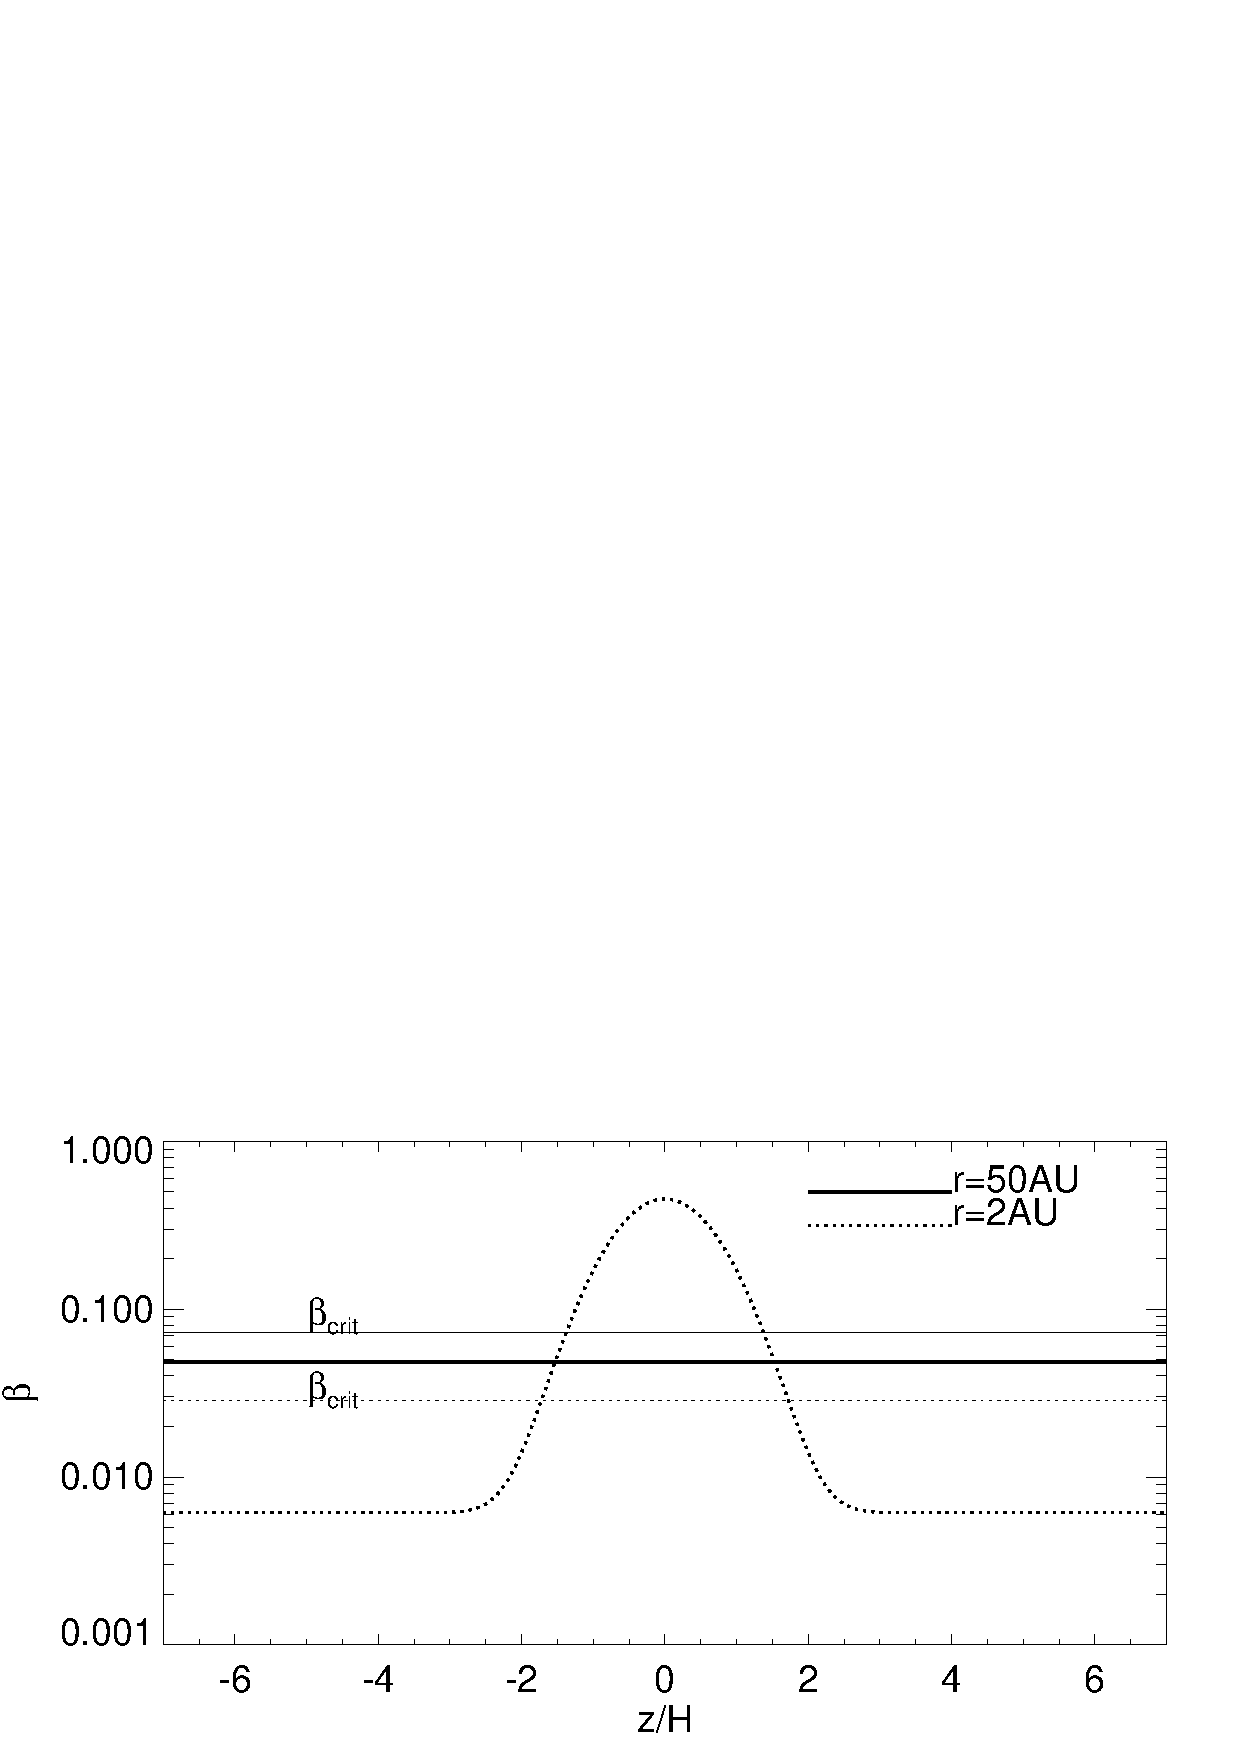
\includegraphics[width=\linewidth,clip=true,trim=0cm 0cm 0cm
  0cm]{figures/beta_compare}
  \caption{Thermal relaxation timescales in the MMSN at $r=50$AU
    and $r=5$AU for $\khat=30$ (solid lines). The
    corresponding horizontal dashed lines are the critical thermal
    relaxation timescales derived in linear theory. 
    \label{beta_compare}}
\end{figure}











In Fig. \ref{mmsn_bcrit_bcool} we compare the above thermal timescale,
Eq. \ref{beta_mmsn_simp},  for several opacity scales, to  
the VSI criterion Eq. \ref{iso_vsi_cond} evaluated for the MMSN,     
\begin{align}\label{bcrit_mmsn}
  % \beta_\mathrm{crit} = \frac{1.44\times10^{-2}}{(\gamma
  % -1)}\left(\frac{\hat{T}}{\mu}\right)^{1/2}r_\mathrm{AU}^{2/7}. 
  \beta_\mathrm{crit} = 0.024r_\mathrm{AU}^{2/7}. 
\end{align}


\begin{figure*}
  \includegraphics[scale=.47,clip=true,trim=0cm 1.8cm 0cm
  0cm]{figures/bcrit_mmsn_kap0d1_z0}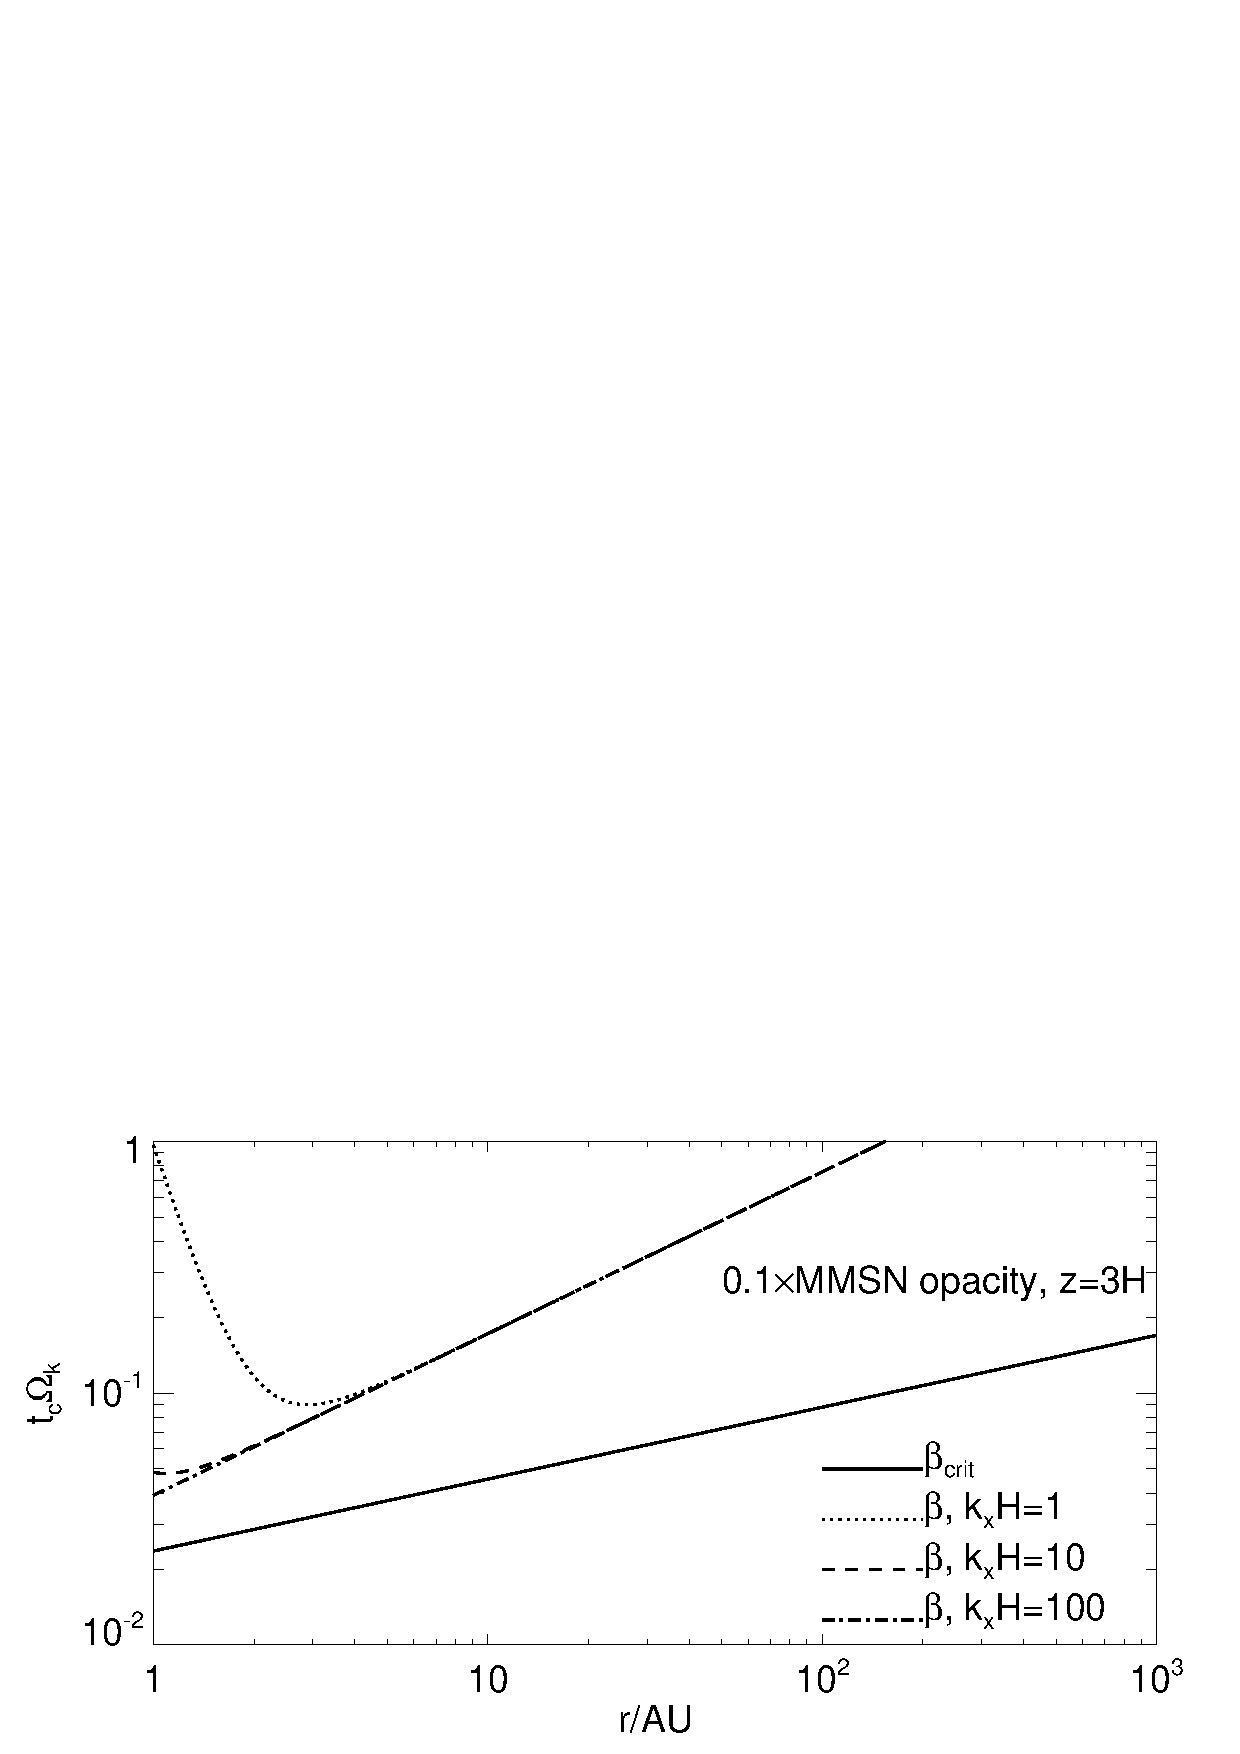
\includegraphics[scale=.47,clip=true,trim=2.5cm 1.8cm 0cm
  0cm]{figures/bcrit_mmsn_kap0d1_z3}\\ 
  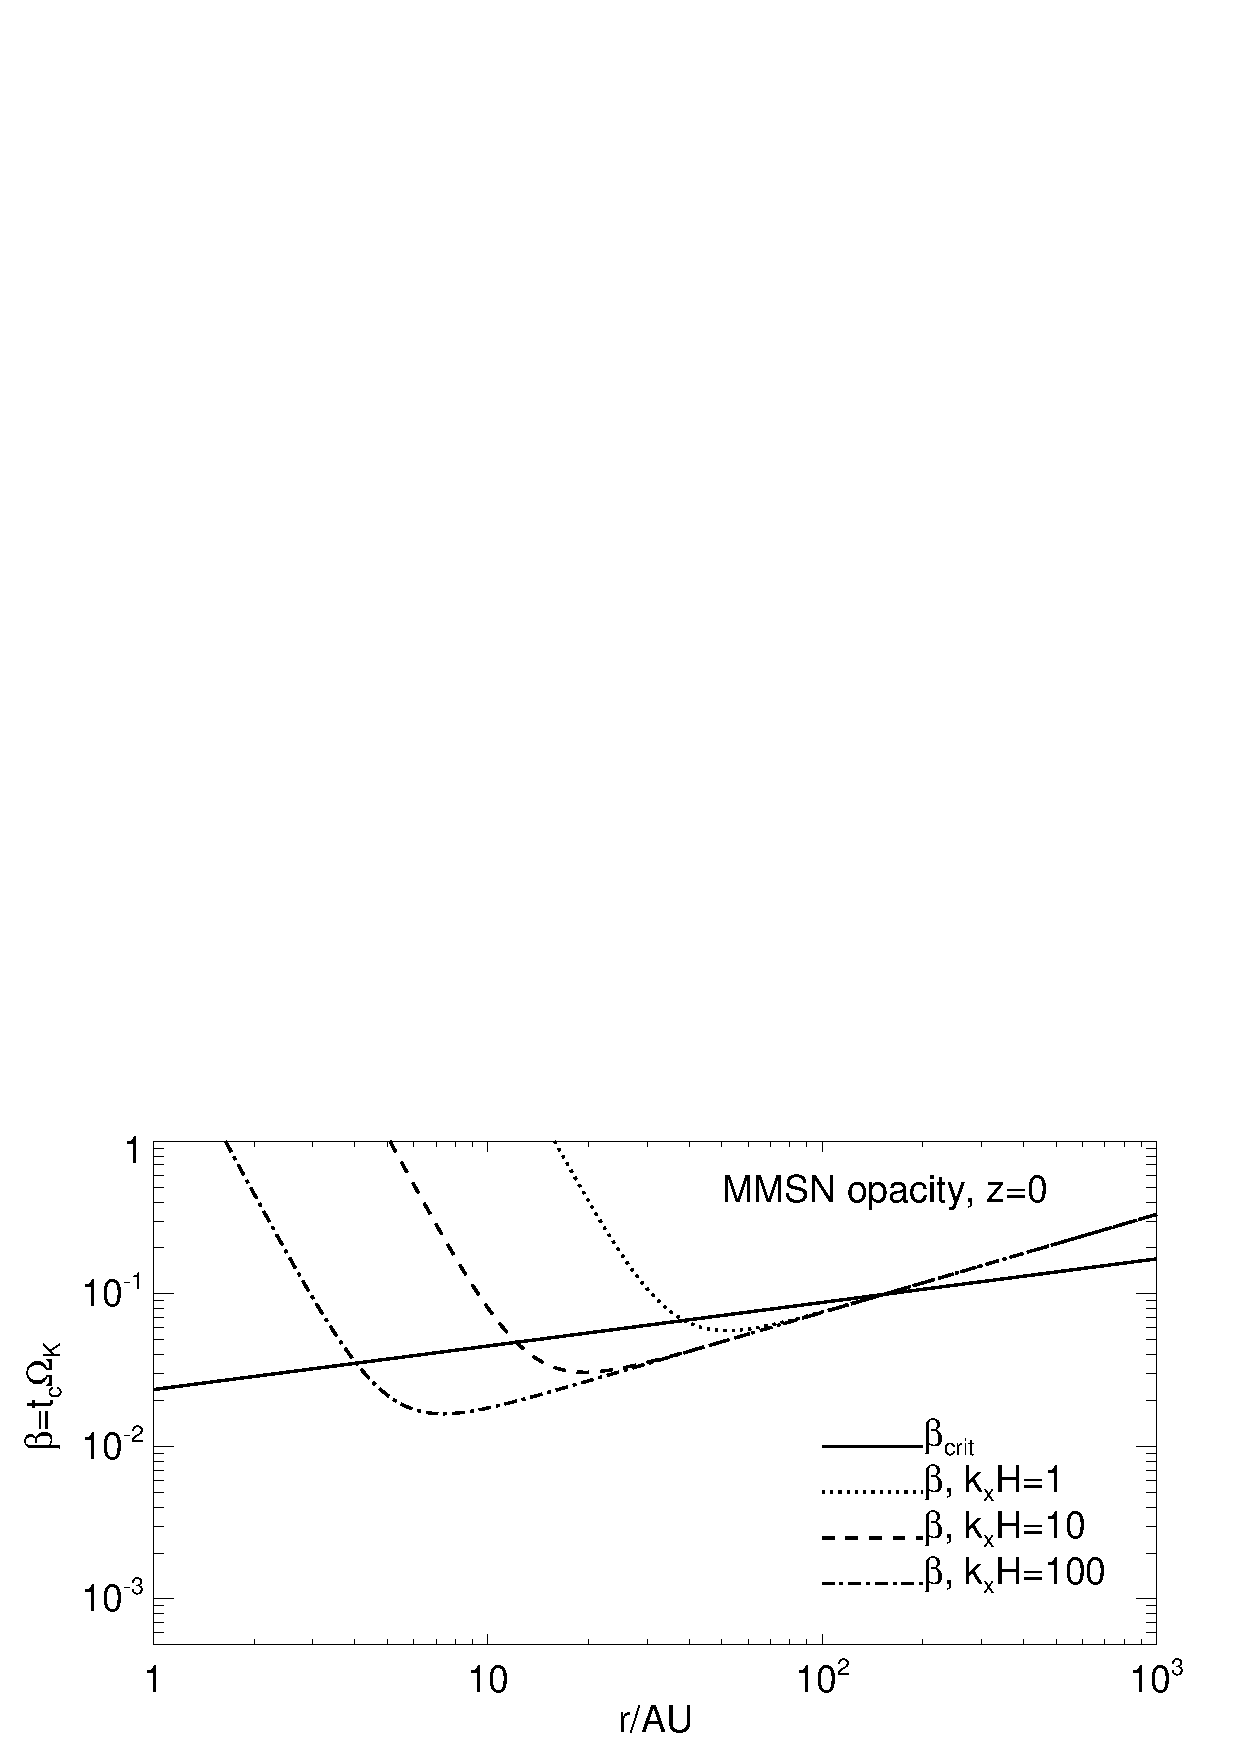
\includegraphics[scale=.47,clip=true,trim=0cm 1.8cm 0cm
  1cm]{figures/bcrit_mmsn_kap1_z0}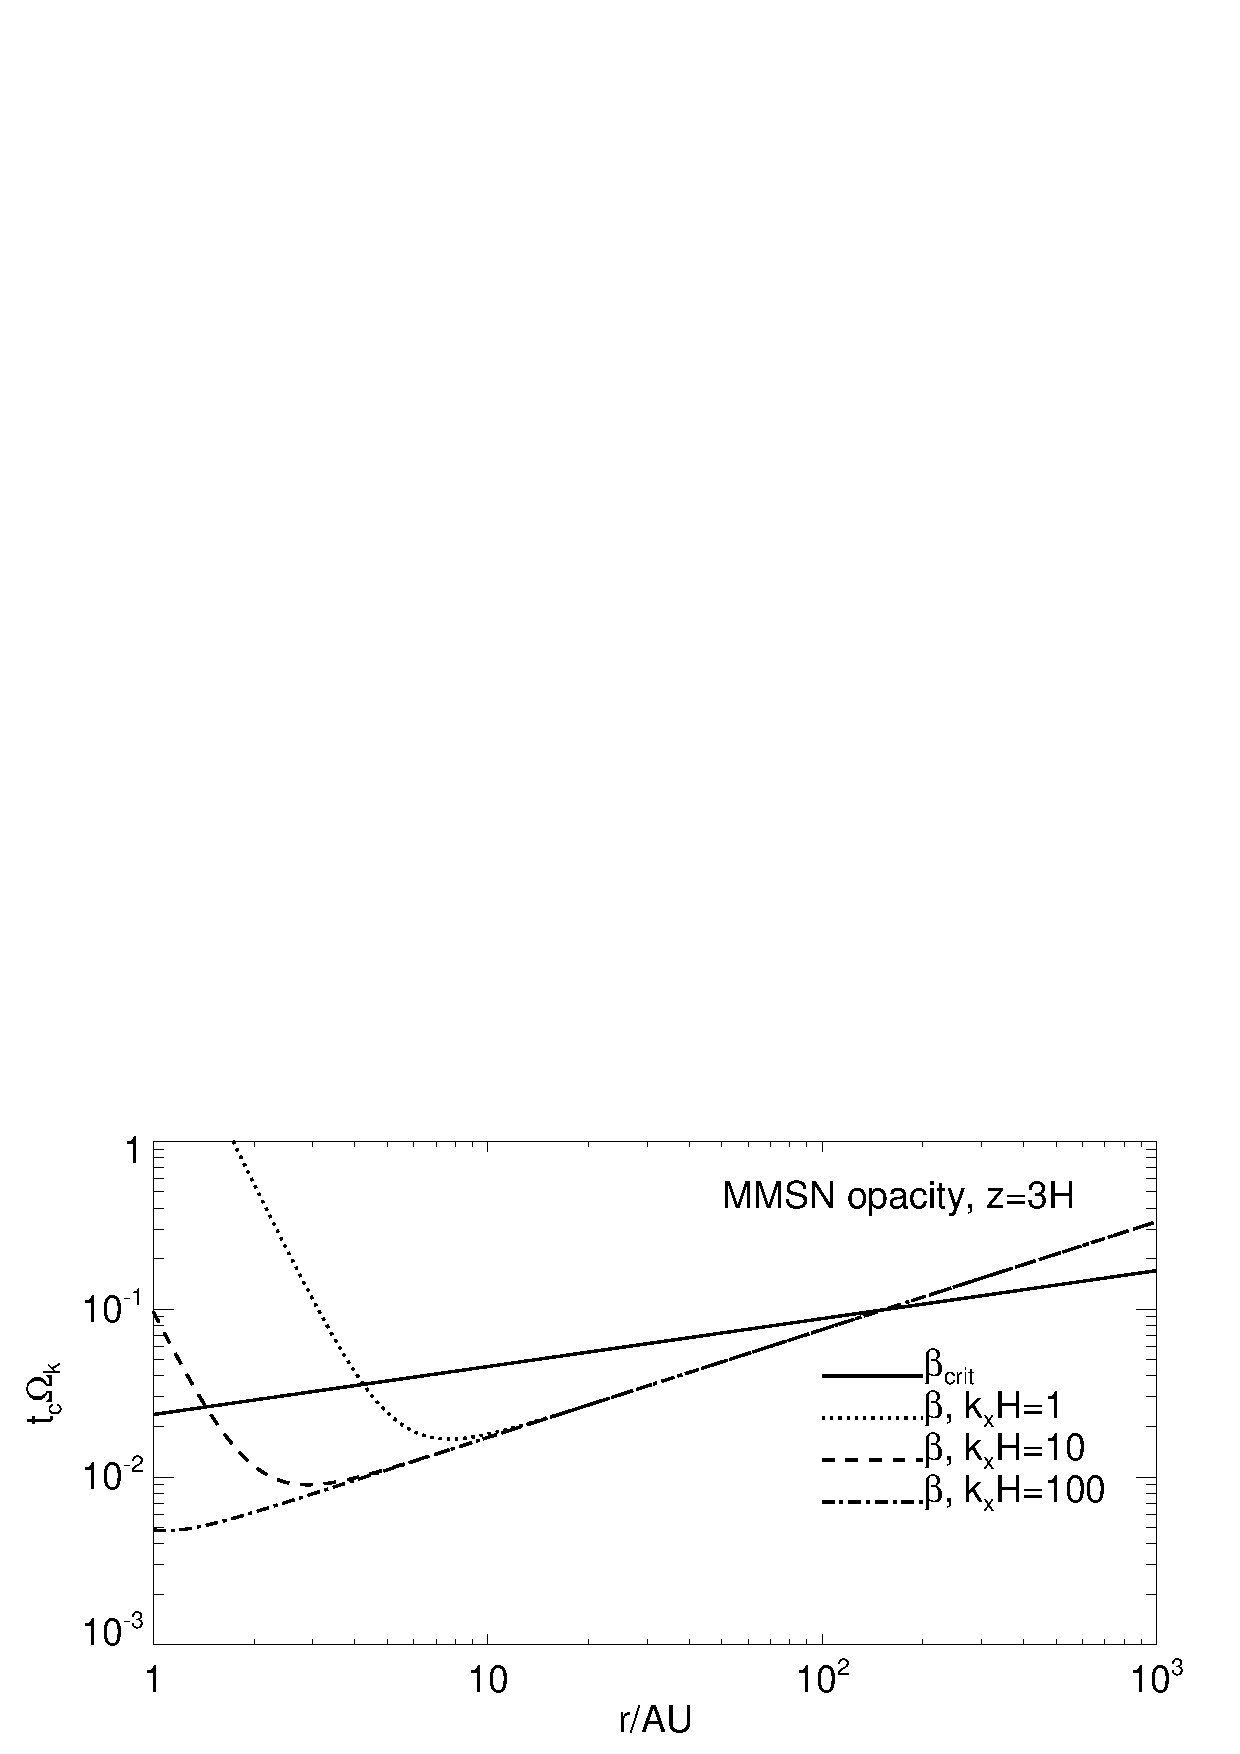
\includegraphics[scale=.47,clip=true,trim=2.5cm
  1.8cm 0cm 1cm]{figures/bcrit_mmsn_kap1_z3}\\
  \includegraphics[scale=.47,clip=true,trim=0cm 0cm 0cm
  1cm]{figures/bcrit_mmsn_kap10_z0}\includegraphics[scale=.47,clip=true,trim=2.5cm 0cm 0cm
  1cm]{figures/bcrit_mmsn_kap10_z3} 
  \caption{Dimensionless thermal relaxation timescales $\beta$,
    evaluated at the midplane (left) and at $z=3H$ (right) in the
    fiducial PPD. Eq. \ref{beta_mmsn_simp} is plotted  
    for three values of the 
    perturbation radial wavenumber: $\khat=1$ (dotted), $\khat=10$
    (dashed) and $\khat=100$ (dashed-dot), for three values of the
    opacity relative to the MMSN: $\hat{\kappa}_d=0.1$ (top),
    $\hat{\kappa}_d=1$ (middle) and $\hat{\kappa}_d=10$ (bottom).  
    The solid line is the 
    critical thermal relaxation timescale $\beta_\mathrm{crit}$.  
    \label{mmsn_bcrit_bcool}}   
\end{figure*}  


For disturbances in the optically-thin cooling regime, $\beta$ does
not depend on the height $z$ or perturbation lengthscale $\khat$. This
generally occurs at sufficiently large radii. In this case we may
directly compare $\beta$ to $\beta_\mathrm{crit}$, which was derived
assuming it is vertically-uniform.  For the case with MMSN
opacity ($\hat{\kappa}_d=1$), we  infer that the VSI can operate at
10s of AU.   

For disturbances in the optically-thick or diffusive regime, $\beta$
increases with decreasing $\khat$ (larger scales) and decreases with
increasing height, on account of the density-dependence of
$t_\mathrm{diff}$.  This generally occurs at small radii. In this case 
$\beta$ may be smaller or greater than $\beta_\mathrm{crit}$ depending
on $z$. Our analytical criteria $\beta < \beta_\mathrm{crit}$ is not valid for
vertically non-uniform $\beta$, and we must turn to numerical
solutions of the linear problem to determine whether or not the VSI
operates. We do this in \S\ref{vsi_mmsn_grow}.  



%\emph{a better organized discussion might end on this point.  Might not be easy to rearrange to do this, but it would ideal to have the seamless flow to what you do next.}
 
Next consider the effect of the opacity scale $\hat{\kappa}_d$. The previous section
(see also Eq. \ref{beta_mmsn_simp}) indicates that increasing $\hat{\kappa}_d$
increases (decreases) the cooling time in the optically thick (thin)
limits. The overall effect of  increasing (decreasing) the opacity
scale by an order of magnitude is illustrated in the lower (upper)
panels of Fig. \ref{mmsn_bcrit_bcool}. 

For increasing opacity, $\hat{\kappa}_d=1\to 10$,  a comparison
between the middle and lower panels shows that the optically-thick
regions shift outward (where the three curves are distinct); while the
optically-thin regions have lowered cooling times (where the curves
overlap). Thus, instability is expected to be restricted to larger
radii. 

For decreasing opacity, $\hat{\kappa}_d=1\to 0.1$,  the
optically-thick regions shift inwards; while cooling times in the
optically-thin limit are increased. In fact, the latter effect is
significant enough to raise $\beta > \beta_\mathrm{crit}$ over all
radii, and even away from the midplane. This is expected to stabilize
the disk against the VSI.  




%\emph{the following statement is not generally true, so it should not be stated without caveat}

We remark that it is possible to satisfy $\beta < \beta_\mathrm{crit}$
at small radii for sufficiently large $\khat$. We illustrate this in 
Fig. \ref{mmsn_bcrit_bcool_mink} by plotting at each radius the value
of $\khat$ such that $\beta = \beta_\mathrm{crit}$. If we consider the
midplane at, say $r\sim 1$AU, the VSI would only occur on very small
radial lengthscales $\ll O(10^{-2}H)$. It is, however, unclear if such
small-scale disturbances are dynamically important.  

%In the disk
% atmosphere where $\beta$ is small, surface modes may develop, 
% but they are not well-defined in vertically isothermal disk models
% with an imposed boundary, and they also require large $\khat$. 

\begin{figure}
  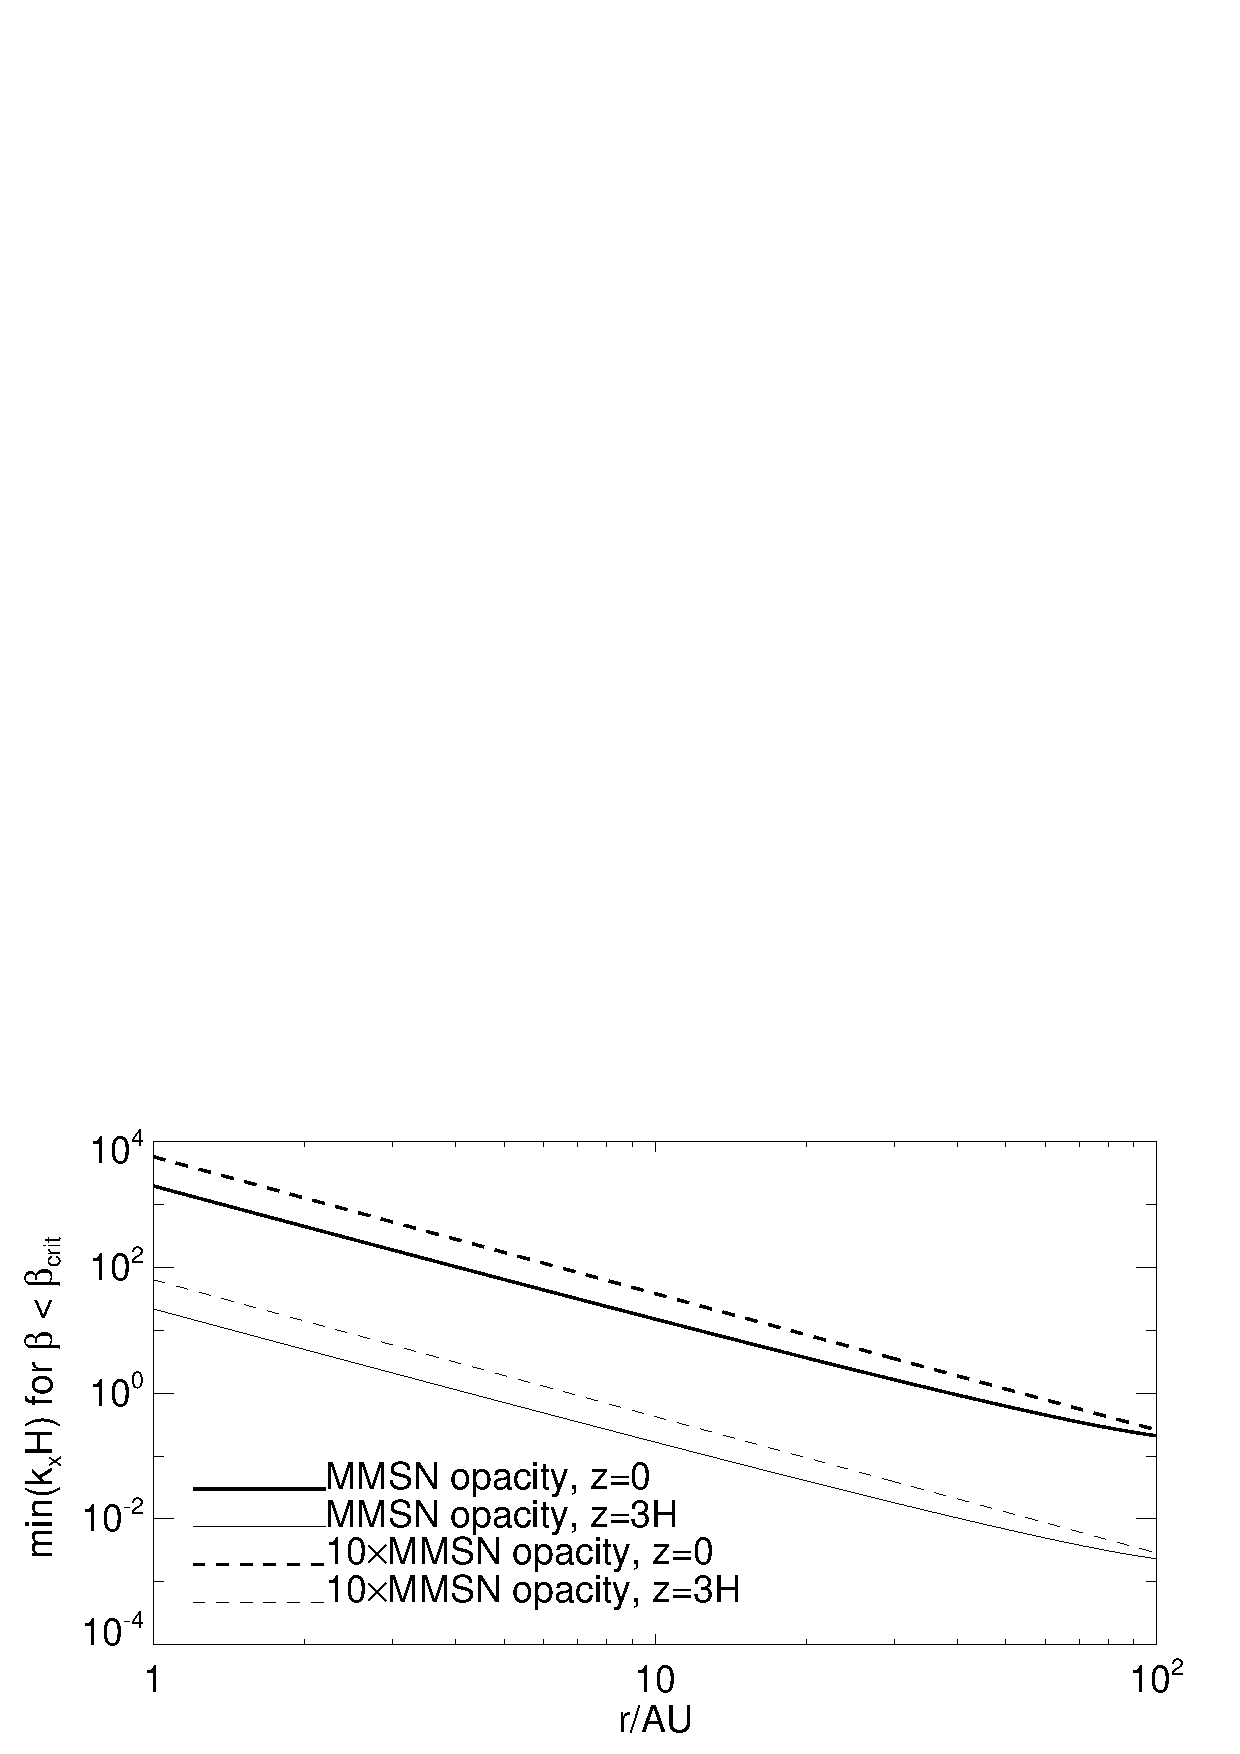
\includegraphics[width=\linewidth]{figures/bcrit_mink} 
  \caption{The minimum perturbation wavenumber $\khat$ in
    the MMSN such that the associated dimensionless thermal
    relaxation time $\beta$ at $z=0$ (solid) and $z=3H$ (dashed) is
    less than the critical timescale $\beta_\mathrm{crit}$.   
    \label{mmsn_bcrit_bcool_mink}}   
\end{figure}  

\subsection{VSI growth in the MMSN}\label{vsi_mmsn_grow}
Here we solve the linear stability problem in the MMSN with the scale and
height dependent thermal relaxation timescale given by
Eq. \ref{beta_mmsn_simp}. 

% \\
% \emph{For this figure to belong here (and not in the previous subsection, with the other comparisons of $\beta$ and $\beta_{crit}$) the discussion should be be more focused on the linear analysis.  Again it's better to start by discussing what the figure tells us, than repeating the figure caption. E.g.\ you could use Fig 21 to explain when a height varying $\beta$ is required.  I would also explain (especially if it stays in this subsection) what the growth time is for the r = 5 AU case.  Looks to be $\sim 1000$ orbits, which is remakrable given that $\beta < \beta_{\rm crit}$ outside $z \gtrsim  1.6 H$.?  That kind of detail could be illuminating, as it's nominally surprising given previous evidence that behavior near 5 -- 7 $H$ can affect growth.}


In Fig. \ref{mmsn_overall} we plot characteristic growth timescales
$t_\mathrm{grow} \equiv 1/\sigma$ of the fundamental mode with a range of
wavenumbers, in units of the local orbital time $P_\mathrm{orb}\equiv
2\pi/\OmK$. In fact, we either only find the fundamental mode, or 
that it is the most unstable, except for the appearance of some 
surface modes for large wavenumbers $\khat\gtrsim 50$. We do not
consider surface modes since they are boundary-dependent and likely
subject to viscous decay (see). 
%  which are 
% boundary-dependent. 
% Disturbances with large $\khat$ are also more likely subject to viscous 
% decay, as discussed above. 
 %\\
%\emph{above sentence too long and complex, could e.g.\ split off that surface modes are neglected and why.}
%However, surface modes are dependent on
%boundary conditions in a vertically isothermal disk \citep{barker15},  
%and 

We therefore consider Fig. \ref{mmsn_overall} as a representation of the
VSI in the fiducial MMSN. We see the VSI operates from $\sim 5$AU to $\sim
50$AU with growth timescales $\sim 30$---40 orbits and
$t_\mathrm{grow}$ rises rapidly towards the inner disk. It is
necessary to consider smaller scales with decreasing $r$ as
perturbations generally become optically thick.   

The fact that we obtain the VSI in the inner disk despite $\beta >
\beta_\mathrm{crit}$ near the midplane suggests that the instability
can operate provided $\beta < \beta_\mathrm{crit}$ for a sufficiently large
fraction of the vertical domain. However, the normalized growth times
become much longer. For example, for $\khat=30$ we find
$t_\mathrm{grow}\sim 40$ orbits at $r=50$AU, but $t_\mathrm{grow}\sim
400$ orbits at $r=5$AU (and rapidly increases to $> 10^3P_0$ for
smaller $r$). Thus, introducing an optically thick midplane
significantly reduces the efficiency of the VSI despite $\beta <
\beta_\mathrm{crit}$ away from the midplane. 

%surface modes may develop for large kx, they are not affected 

We thus find Fig. \ref{mmsn_overall} to be roughly consistent with
comparing the midplane thermal relaxation timescales to the critical
thermal timescale. For example, 
Fig. \ref{mmsn_bcrit_bcool} show that $\beta(z=0,\khat=10) \gtrsim
\beta_\mathrm{crit}$ for $r\lesssim 10$AU in the MMSN (left middle
panel); and Fig. \ref{mmsn_overall} 
show that modes with $\khat=10$ are stabilized inside $\sim 8$AU (where
$t_\mathrm{grow}\to\infty$). Our numerical results suggest the VSI
is efficient at radii of few tens of AU in the MMSN, consistent with
estimates made by \citetalias{nelson13}. 

\begin{figure}
  \includegraphics[width=\linewidth]{figures/eigen_compare_grow.ps}
  \caption{Characteristic growth times of the VSI in 
    the MMSN. These are calculated using the thermal relaxation
    function given by Eq. \ref{beta_mmsn_simp}. 
    \label{mmsn_overall}}    
\end{figure}
